\section{Resultados estruturais}

Ao final do projeto cerca de 90\% da estrutura da estufa foi fabricada pelos estudantes, onde os outros 10\% eram partes que levariam muito trabalho técnico e poderia, consequentemente, atrasar o cronograma do projeto. A seguir tem-se os materiais utilizados para cada um e como se deu o processo de fabricação.
\subsection{Estrutura interna}
Materiais
\begin{itemize}
	\item Cantoneiras
	\item Chapas de alumínio
	\item Corrediças telescópicas
\end{itemize}
Fabricação
\begin{itemize}
	\item As cantoneiras foram soldadas para dar forma ao chassi.
	\item Uma chapa de alumínio foi cortada na cortadora de chapas e em seguida foi rebitada no chassi para fazer o fundo da estrutura.
	\item As corrediças telescópicas foram presas no chassi com parafusos, e tais furos foram feitos com a fresadora.
	\item Uma outra chapa de alumínio foi cortada na cortadora de chapas e em seguida dobrada na dobradeira de chapas para fazer a gaveta onde comportará as mudas.
	
\end{itemize}

As figuras de \ref{fig:estrutura_interna1} a \ref{fig:estrutura_interna3} apresentam os resultados da estrutura interna.
\begin{figure}[!htb]
	\centering
	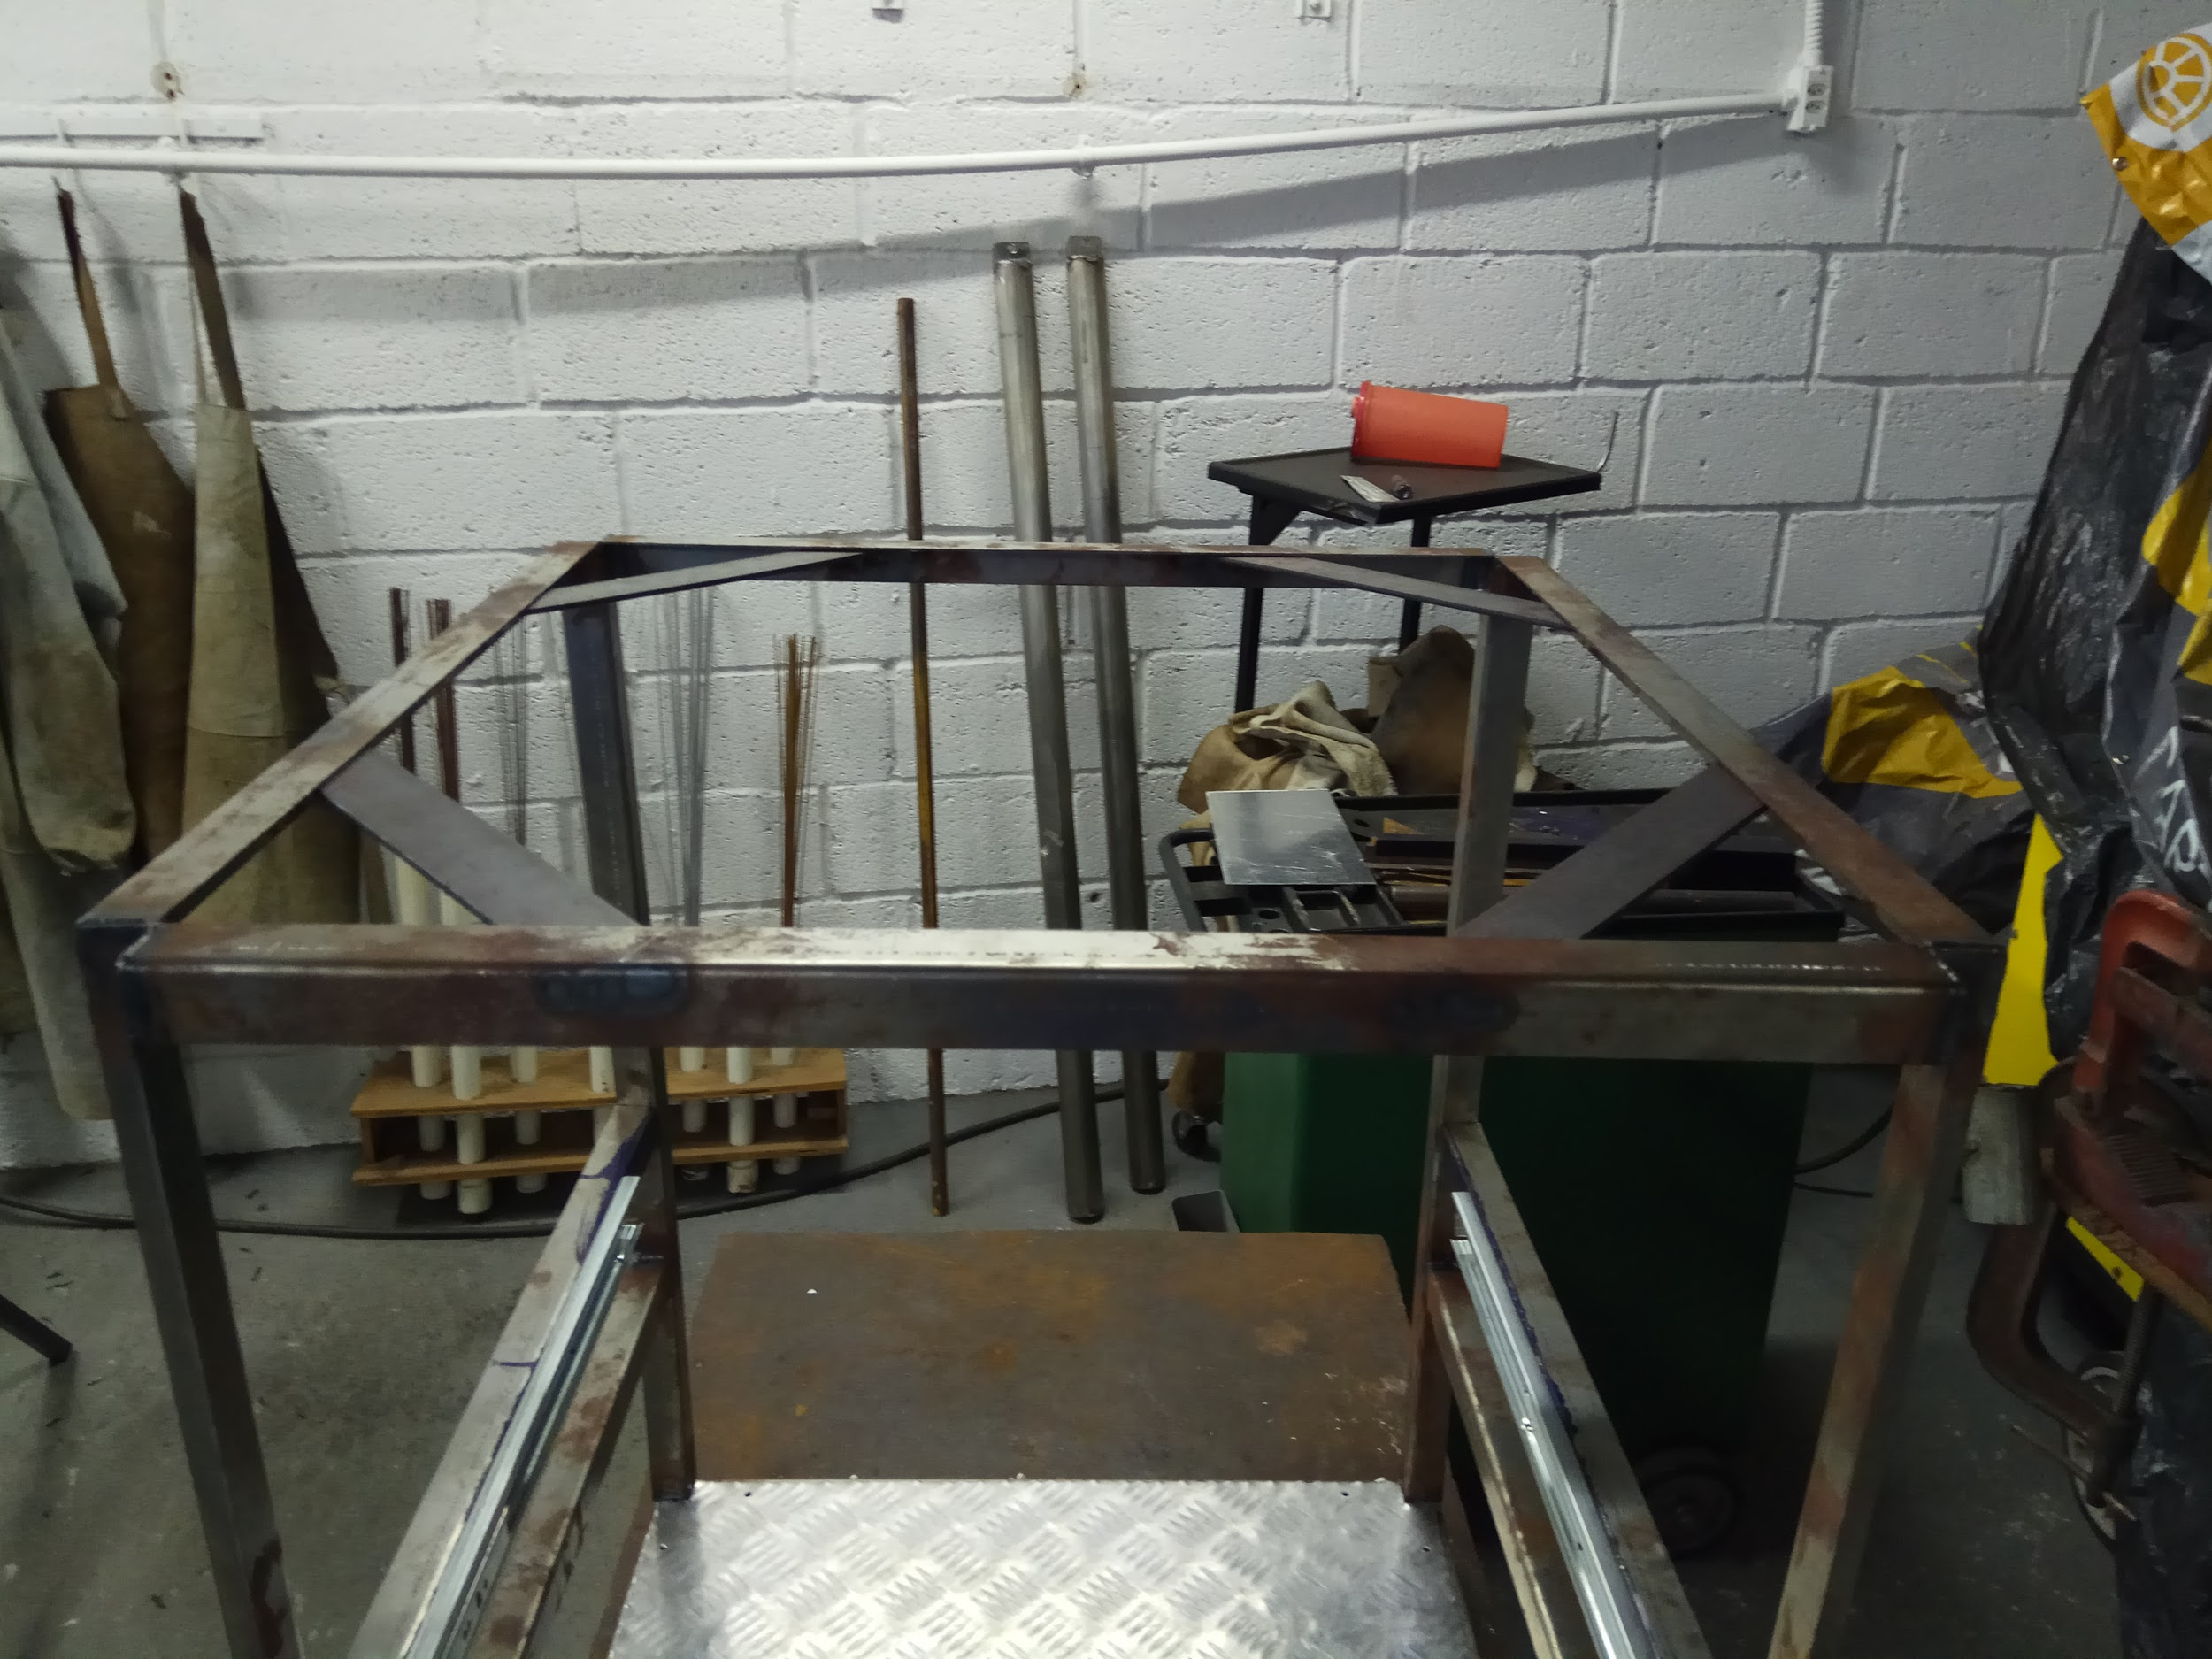
\includegraphics[width=10cm]{figuras/estrutura_interna1.png}
	\caption{Parte superior da estrutura interna}
	\label{fig:estrutura_interna1}
\end{figure}
\begin{figure}[!htb]
	\centering
	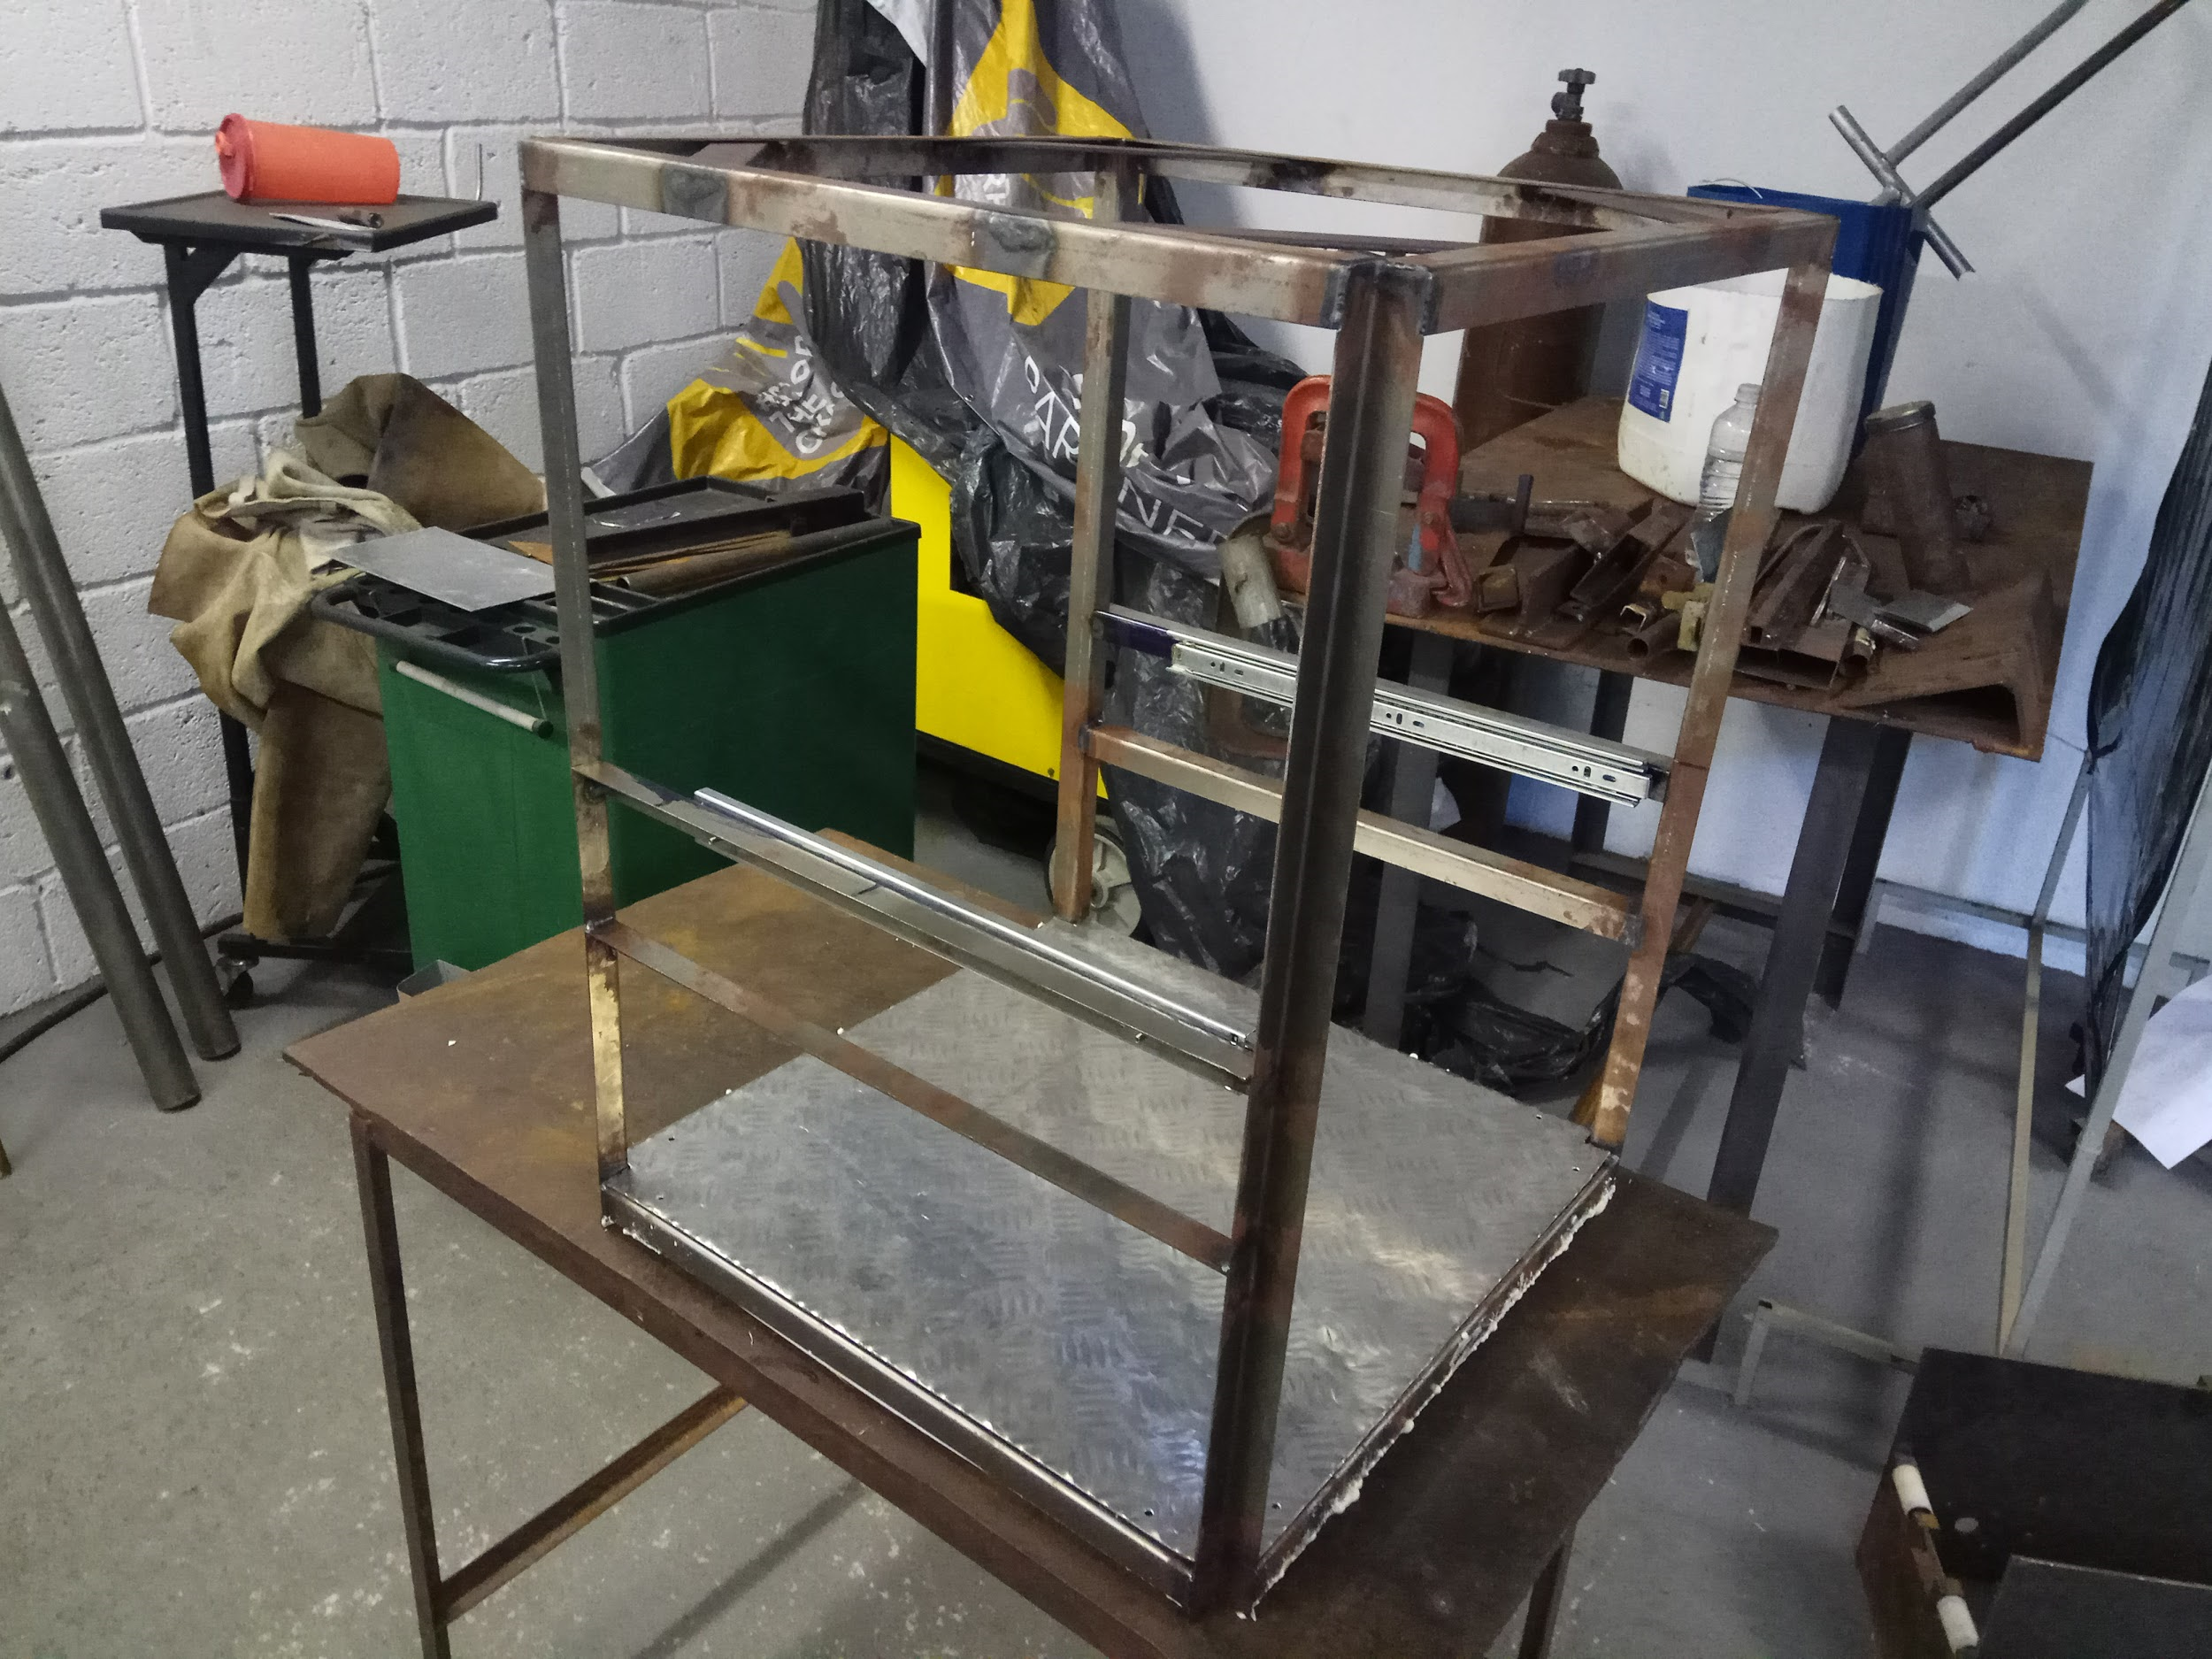
\includegraphics[width=10cm]{figuras/estrutura_interna2.png}
	\caption{Estrutura interna de perfil}
	\label{fig:estrutura_interna2}
\end{figure}
\begin{figure}[!htb]
	\centering
	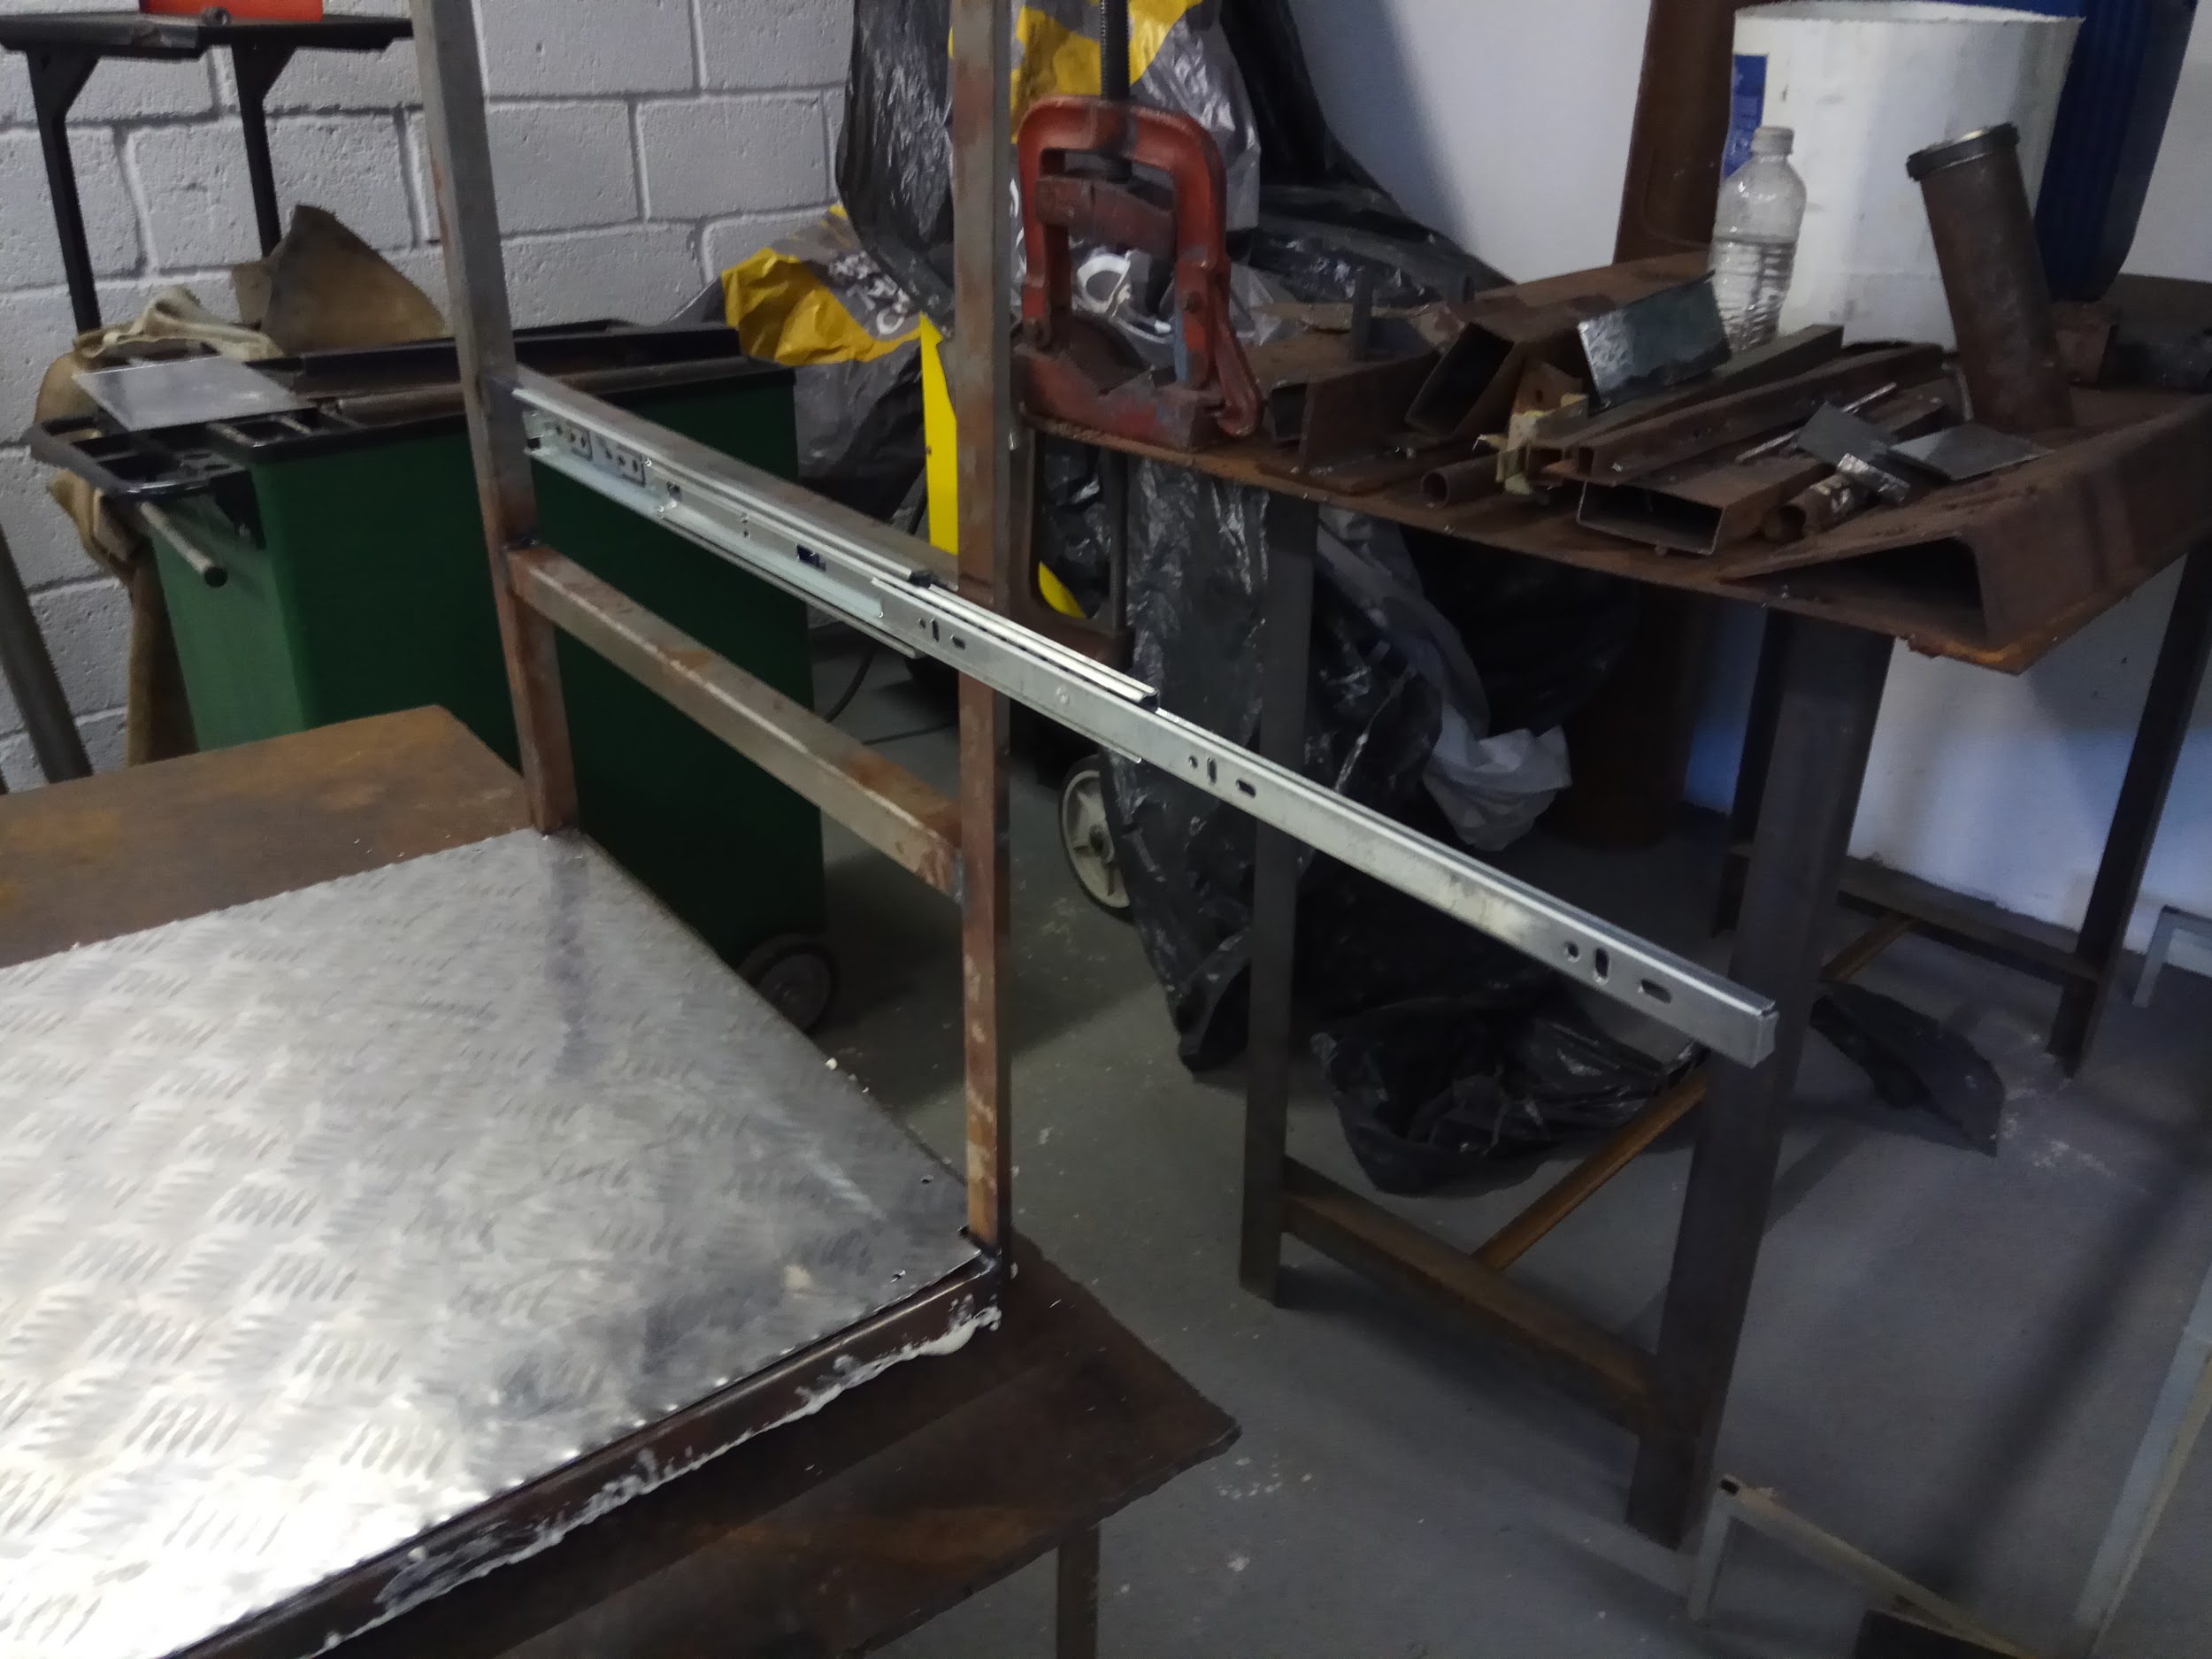
\includegraphics[width=10cm]{figuras/estrutura_interna3.png}
	\caption{Corrediça telescópica onde comportará a gaveta de mudas}
	\label{fig:estrutura_interna3}
\end{figure}
\subsection{Porta}

A porta da estufa foi a única parte do projeto estrutural na qual foi terceirizada a construção, não por motivos de competência da equipe, mas pensando em prazos apertados e em busca de um melhor acabamento final, figura \ref{fig:porta}. Para obter uma boa resistência estrutural utilizou-se o alumínio como material. Além disso, para que o usuário da estufa possa ver o seu interior usou-se vidro em sua maior parte. Para que não haja trocas de ar interno e externo sem que seja necessário há uma espuma de vedação na porta, onde ao fechar faz um isolamento.

\begin{figure}[!htb]
	\centering
	\includegraphics[width=10cm]{figuras/porta.png}
	\caption{Porta da estufa}
	\label{fig:porta}
\end{figure}

Materiais

\begin{itemize}
	
	\item Alumínio
	\item Vidro laminado
\end{itemize}

\subsection{Estrutura externa}
Materiais
\begin{itemize}
	\item MDF
	\item Isopor
	\item PVC
	\item Silicone
	\item Espuma Expansiva
	\item Forro PVC
	\item Alça
\end{itemize}
Fabricação
\begin{itemize}
	\item Foram realizadas medições da estrutura do Chassi, onde serão colocadas chapas de MDF para cobrir a estrutura, deixando a estrutura mais resistente, com um aspecto visual mais requintado. Na parte superior da estrutura, decidiu-se colocar MDF para fixar as lâmpadas, visto que anteriormente utilizaria isopor, porém por questão de segurança decidiu-se fazer esta alteração.
	\item Antes das chapas de MDF, foram alocadas placas de isopor como revestimento interno, onde foram cortados os espaços e instalaram-se alguns componentes como os Coolers nas laterais da estufa.
	\item Na parte externa foram cortadas placas de PVC de tamanho adequado, para compor a parte externa da estufa.
	\item Foram utilizados silicone e espuma expansiva para realizar a junção das partes e para realizar o isolamento térmico da parte interna da estrutura.
	\item Adicionou-se na estufa folhas de alumínio para que se tenha a máxima eficiência luminosa, onde foram cortadas e presas nas laterais.
	\item O isopor foi cortado do tamanho da estrutura para fazer o isolamento térmico. Além disso utilizou-se o PVC para dar um isolamento extra e maior resistência ao isolamento. Ao todo foram três camadas de isopor e uma de PVC.
	\item Forros de PVC foram utilizados na parte mais externa da estufa para dar um melhor acabamento e, consequentemente, uma maior resistência estrutural. Com isso, foram cortadas as placas de forro e parafusadas na estrutura.
	\item Para poder movimentar a estufa mais facilmente foram colocadas duas alças de metal nas laterais para poder fazer o transporte da estuda se necessário, em seguida foram parafusadas.
	
\end{itemize}

As figuras \ref{fig:isolamento1} e \ref{fig:isolamento2} apresentam a partem de isolamento térmico da estufa, a figura \ref{fig:isolamento3} mostra a estufa após a instalação dos forros PVC e das alças e a \ref{fig:folha_aluminio} as folhas de alumínio instaladas.
\begin{figure}[!htb]
	\centering
	\includegraphics[width=10cm]{figuras/isolamento1.png}
	\caption{Estrutura com isolamento térmico}
	\label{fig:isolamento1}
\end{figure}
\begin{figure}[!htb]
	\centering
	\includegraphics[width=10cm]{figuras/isolamento2.png}
	\caption{Estrutura com o isolamento externo}
	\label{fig:isolamento2}
\end{figure}
\begin{figure}[!htb]
	\centering
	\includegraphics[width=10cm]{figuras/isolamento3.png}
	\caption{Estrutura após a instalação dos forros e das alças}
	\label{fig:isolamento3}
\end{figure}
\begin{figure}[!htb]
	\centering
	\includegraphics[width=10cm]{figuras/folha_aluminio.jpg}
	\caption{Folhas de alumínio instaladas nas laterais da estufa}
	\label{fig:folha_aluminio}
\end{figure}
\subsection{Estrutura final}
\begin{figure}[!htb]
	\centering
	\includegraphics[width=10cm]{figuras/estufapreta_frente.JPG}
	\caption{Estrutura final vista de frente}
	\label{fig:estufapreta_frente}
\end{figure}
\begin{figure}[!htb]
	\centering
	\includegraphics[width=10cm]{figuras/estufapreta_cima.jpg}
	\caption{Estrutura final vista de cima}
	\label{fig:estufapreta_cima}
\end{figure}
\begin{figure}[!htb]
	\centering
	\includegraphics[width=10cm]{figuras/estufapreta_lado.JPG}
	\caption{Estrutura final vista de lado}
	\label{fig:estufapreta_lado }
\end{figure}
